	\section{Simulation der Widerstandsmatrix}
	Ebenfalls wurden die drei Leistungsstufen mit den SMD-Widerst�nden realisiert. Dabei ist die Aufgrund der geringeren Gr��e eine h�here leistungsgleiche realisiert werden. Die Simulation der Drei Leistungen mit einem Ausgangsabstand von 2 mm ergab folgende Temperaturen:
		
	\begin{center}
		\begin{minipage}[!ht]{1.0\textwidth}
			\captionsetup{type=table}
			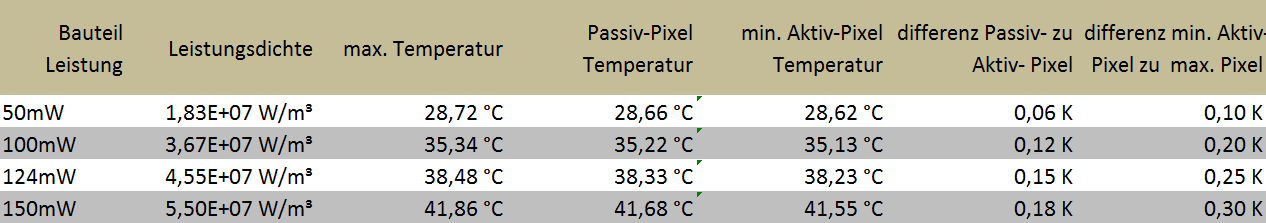
\includegraphics[width=1\linewidth]{bilder/Unbenannt}
			\caption{Statische Ergebnisse}
			\label{tab:Tabelle_Statische_ergebnisse}
		\end{minipage}
	\end{center}
	
		\subsection{Optimierung}
		Ziel einer Optimierung ist es nun, die Temperaturdifferenz von zwei Pixeln und dem Bereich zwischen diesen Pixeln so gering wie m�glich zu halten. Jedoch ist dabei der Mindestabstand zwischen den Pixeln zu betrachten. Durchgef�hrt wurde die Optimierung mit 124 mW Bauteilleistung. Grund daf�r ist, dass in einer vorherigen Optimierung versucht wurde die typische Temperatur einer Maus zu erreichen. Ergebnis war, das diese Temperatur mit 124 mW ann�hernd erreicht wurde. Der Abstand Zwischen den Pixeln hatte bei der durchgef�hrten Optimierung nur geringen Einfluss auf die Pixeltemperaturen. Folgendes Ergebnisbild entstand mit den Optimalen Ergebnissen.
		
		\begin{center}
			\begin{minipage}[!ht]{0.6\textwidth}
				\captionsetup{type=figure}
				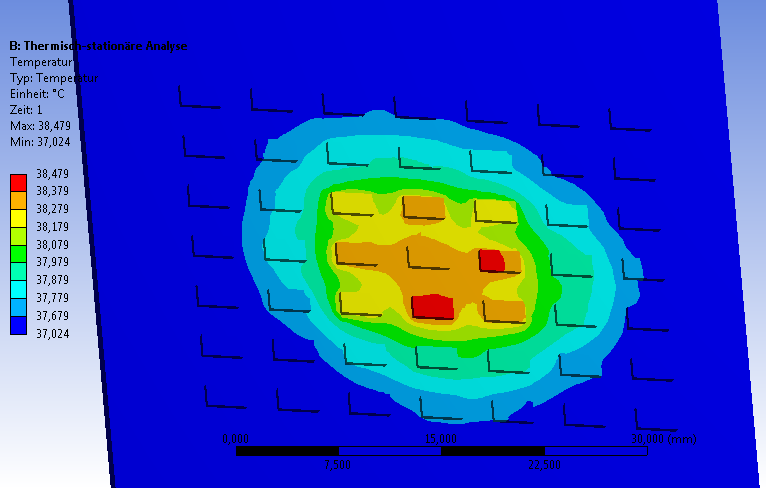
\includegraphics[width=1\linewidth]{bilder/Widerstand_124mW_laut_opti_3,94}
				\caption{Optimierungsergebnis Widerstandsmatrix}
				\label{fig:Optimierungsergebniss_Widerstandsmatrix}
			\end{minipage}
		\end{center}
		
		Da der Mindestabstand (L�ckengr��e) in Y Richtung 1,6 mm betr�gt, Ist dies der Startwert. Laut Optimierung ergibt sich bei einer L�ckengr��e von 2,38 mm eine minimale Temperaturdifferenz. Jedoch wie die Abbildung \ref{fig:Optimierungsergebniss_Widerstandsmatrix} zeigt, Ist auch bei diesem wert eine Relativ Gro�e Temperaturdifferenz zu erkennen. Um Die Differenz zu veranschaulichen wurden die Farben mit 0,1 �C bez�glich der Maximaltemperatur abgestuft.
		
		Die Simulationsergebnisse k�nnen jedoch von der Realit�t abweichen, da keine Luftbewegung in der Simulation ber�cksichtigt wird. Weiter beeinflussen andere Faktoren wie Umgebungstemperatur und Luftfeuchtigkeit das Ergebnis.
		\subsection{Aufgabe mit Rand}
		Laut Aufgabenstellung ist ein versuch gefordert der folgende Aufteilung besitzt. Dabei wurde das innere Rechteck mit 50 mW Simuliert, dies sollte daf�r sorgen das der Au�enring klar erkennbar ist.
		
		\begin{center}
			\begin{minipage}[!ht]{0.8\textwidth}
				\captionsetup{type=figure}
				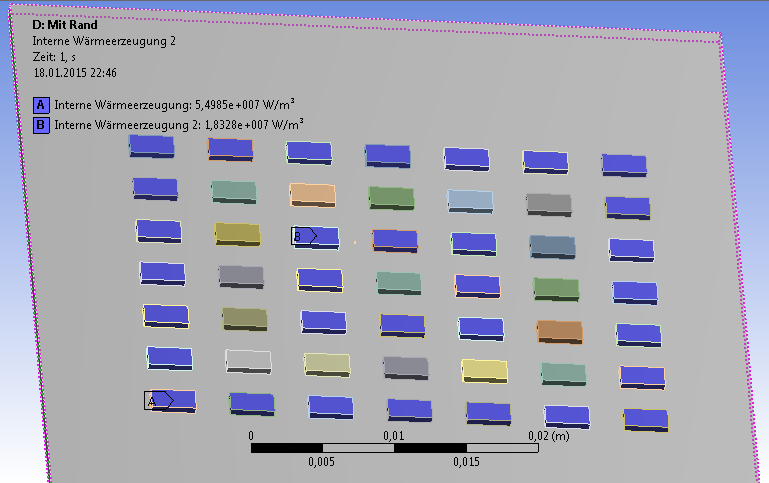
\includegraphics[width=1\linewidth]{bilder/Vorgabe}
				\caption{Vorgabe Versuch mit Ring}
				\label{fig:Vorgabe_Ring}
			\end{minipage}
		\end{center}
		
		Die Abbildung \ref{fig:Ergebnis_Ring} zeigt, dass sich die Platine und die Bauelemente gleicherma�en erw�rmen. das macht es nicht m�glich die Erw�rmungsquellen zu lokalisieren. Weiter zeigt es ,dass die Simulation von der Realit�t abweichen kann.
		
		\begin{center}
			\begin{minipage}[!ht]{0.8\textwidth}
				\captionsetup{type=figure}
				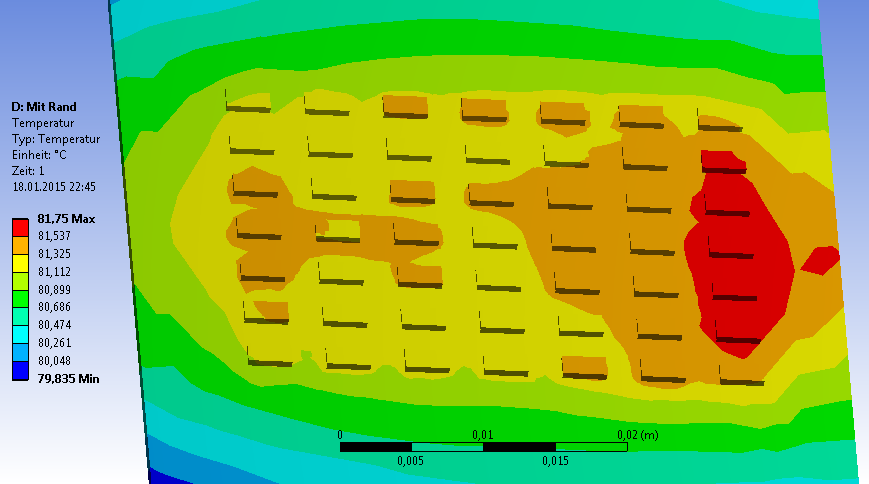
\includegraphics[width=1\linewidth]{bilder/RingErgebniss}
				\caption{Ergebnis Versuch mit Ring}
				\label{fig:Ergebnis_Ring}
			\end{minipage}
		\end{center}